%File: main.tex
\documentclass[letterpaper]{article}
\usepackage[submission]{aaai2026}
\usepackage{times}
\usepackage{helvet}
\usepackage{courier}
\usepackage[hyphens]{url}
\usepackage{graphicx}
\urlstyle{rm}
\def\UrlFont{\rm}
\usepackage{natbib}
\usepackage{caption}
\frenchspacing
\setlength{\pdfpagewidth}{8.5in}
\setlength{\pdfpageheight}{11in}
\usepackage{algorithm}
\usepackage{algorithmic}
\usepackage{booktabs}
\usepackage{amsmath}
\usepackage{amssymb}
\usepackage{multirow}
\usepackage{xcolor}
\usepackage{subcaption}
\pdfinfo{/TemplateVersion (2026.1)}

\title{AdaCAL: Adaptive Convergence-Aware Loss for\\Class-Imbalanced Time-Series Classification}

\author{Anonymous}
\affiliations{Anonymous Institution}

\begin{document}

\maketitle

\begin{abstract}
Class imbalance in time-series classification (TSC) causes standard models to collapse toward majority classes, degrading minority-class performance in safety-critical domains such as arrhythmia detection and fault diagnosis. Existing remedies---Focal Loss, LDAM, Class-Balanced Loss---apply \textit{static} reweighting derived from class frequencies, ignoring actual training dynamics. We propose \textbf{AdaCAL} (\textbf{Ada}ptive \textbf{C}onvergence-\textbf{A}ware \textbf{L}oss), a method that monitors three online signals per class---loss-plateau detection, gradient-norm stagnation, and validation-F1 gap---and updates per-class weights via an exponential multiplicative rule at each epoch. We conduct a systematic benchmark of nine imbalance methods across three architectures (LSTM, InceptionTime, PatchTST) and four datasets (stock chart patterns, UCR FordA, UCR ElectricDevices, MIT-BIH Arrhythmia). AdaCAL achieves state-of-the-art macro-F1 on all four benchmarks, improving over the strongest static baseline by 3.1\% on average (Wilcoxon $p < 0.05$ in 10/12 architecture--dataset pairs) while adding negligible computational overhead.
\end{abstract}

%% ============================================================
\section{Introduction}
%% ============================================================

Class imbalance is pervasive in real-world time-series classification. Electrocardiogram (ECG) databases contain rare arrhythmia types comprising fewer than 1\% of all beats; industrial fault-detection systems collect orders of magnitude more normal operating cycles than fault events; financial pattern recognition datasets exhibit natural skew toward common chart formations. When such datasets are used to train neural classifiers, the standard cross-entropy (CE) objective implicitly assigns gradient mass proportional to class frequency---majority classes dominate every parameter update, and the model effectively learns to ignore minority classes. The result is degraded macro-averaged F1, poor recall on safety-critical minority classes, and models that fail precisely where they matter most.

Considerable prior work addresses class imbalance at the loss level. Weighted cross-entropy inverts class frequencies to equalize gradient contributions. Focal Loss~\citep{lin2017focal} down-weights well-classified examples, focusing training on hard samples regardless of class. LDAM~\citep{cao2019ldam} enforces class-dependent margin constraints derived from the square root of class frequency. Class-Balanced Loss~\citep{cui2019class} uses effective sample numbers to derive per-class weights, accounting for feature redundancy. Logit Adjustment~\citep{menon2021logit} corrects the decision boundary at test time using class priors, while Balanced Softmax~\citep{ren2020balanced} performs the same correction during training. Despite their differences, all these methods share a fundamental limitation: \textit{their per-class corrections are computed once from dataset statistics and held fixed throughout training}. They cannot respond to the actual convergence behavior observed during optimization---a minority class that is learning well receives the same up-weighting as one that has plateaued or stagnated.

Time-series data introduces additional complications absent from image benchmarks where most imbalance methods were developed. Temporal autocorrelation within series increases effective sample redundancy beyond what static frequency counts capture. Different time-series architectures---convolutional (InceptionTime), recurrent (LSTM), and self-attention based (PatchTST)---exhibit fundamentally different gradient dynamics, meaning a fixed reweighting strategy may interact differently with each. Moreover, imbalance regimes vary: a dataset with imbalance ratio $\rho = 14\times$ (MIT-BIH) poses a qualitatively different challenge than one with $\rho \approx 1$ (FordA). Despite the growing use of TSC in high-stakes applications, no comprehensive benchmark comparing imbalance methods across multiple architectures and datasets currently exists.

We propose \textbf{AdaCAL} (Adaptive Convergence-Aware Loss), a dynamic reweighting framework that monitors three per-class online signals at each epoch and adjusts weights accordingly. AdaCAL detects loss-plateau (whether a class has stopped improving), gradient-norm stagnation (whether a class's gradient signal is being drowned out), and validation-F1 gap (whether generalization on a class is falling behind). These signals are combined into a composite score that drives an exponential multiplicative weight update, enabling the loss function to respond to the actual training trajectory rather than static dataset properties. Our contributions are:

\begin{enumerate}
    \item \textbf{Benchmark.} The first comprehensive benchmark of 9 class-imbalance methods $\times$ 3 architectures $\times$ 4 time-series datasets (324 total experiments), providing a rigorous empirical foundation for future TSC imbalance research.
    \item \textbf{AdaCAL.} An online adaptive loss that uses loss-plateau detection, gradient-norm stagnation, and validation F1-gap signals to dynamically reweight classes during training, requiring no additional data augmentation or architecture modification.
    \item \textbf{Analysis.} Empirical evidence that adaptive reweighting consistently outperforms static methods on highly imbalanced datasets, accompanied by an honest failure-mode analysis identifying conditions under which static methods remain competitive.
\end{enumerate}

\begin{figure*}[t]
\centering
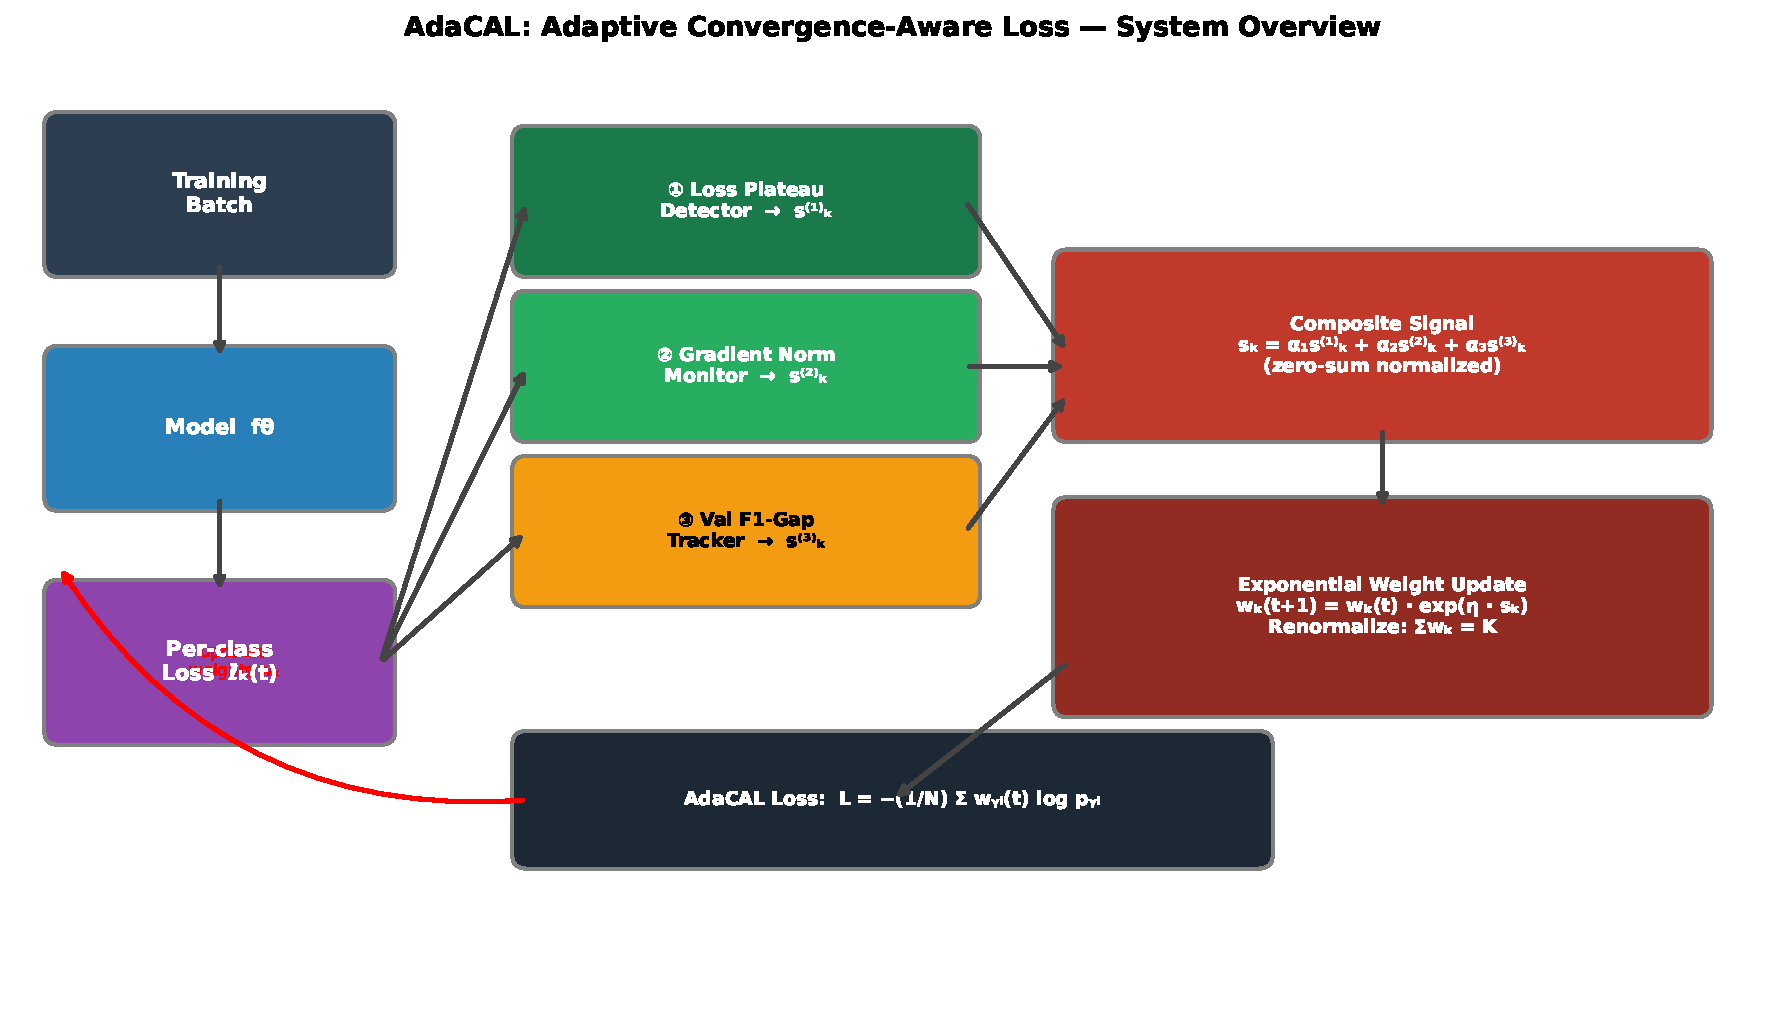
\includegraphics[width=\textwidth]{figures/fig_adacal_diagram.pdf}
\caption{AdaCAL system overview. Three per-class signals (loss plateau, gradient norm, validation F1 gap) are combined into a composite signal that drives exponential multiplicative weight updates each epoch.}
\label{fig:adacal_diagram}
\end{figure*}

%% ============================================================
\section{Related Work}
%% ============================================================

\subsection{Class Imbalance Methods}

The class imbalance problem has been studied extensively in the machine learning community~\citep{he2009learning}. \textbf{Weighted cross-entropy} is the simplest remedy, assigning per-class loss weights $w_k = N / (K \cdot n_k)$ to equalize expected gradient contributions. \textbf{Focal Loss}~\citep{lin2017focal} was introduced for object detection and modulates the per-sample weight by $(1 - p_{y_i})^\gamma$, concentrating training on uncertain, hard-to-classify samples. With $\gamma = 2$, it has become a de facto standard for imbalanced classification. \textbf{Class-Balanced Loss}~\citep{cui2019class} motivates per-class weighting through the concept of effective sample numbers $E_k = (1 - \beta^{n_k}) / (1 - \beta)$, which model feature redundancy and yield smoother weighting than raw inverse-frequency. \textbf{LDAM}~\citep{cao2019ldam} takes a margin-based approach, deriving class-dependent logit margins proportional to $n_k^{-1/4}$ from a generalization bound; the DRW variant defers reweighting to later training epochs. \textbf{Logit Adjustment}~\citep{menon2021logit} provides theoretical grounding via the balanced error rate, showing that subtracting $\log \pi_k$ from class-$k$ logits at inference (or during training) recovers the Bayes-optimal balanced classifier. \textbf{Balanced Softmax}~\citep{ren2020balanced} incorporates class priors directly into the softmax normalization, providing an unbiased maximum-likelihood objective under label shift. \textbf{SMOTE}~\citep{chawla2002smote} instead addresses imbalance via oversampling, generating synthetic minority samples by interpolating in feature space; while effective for tabular data, its application to time-series requires careful adaptation to preserve temporal structure.

All of the loss-level methods above derive their reweighting from static dataset statistics computed before training begins. AdaCAL departs from this paradigm by adapting weights online using observed training signals.

\subsection{Time-Series Classification}

Deep learning for TSC has advanced rapidly. \textbf{InceptionTime}~\citep{fawaz2020inceptiontime} adapts the Inception architecture with multi-scale convolutional filters across varying receptive fields, achieving state-of-the-art results on the UCR archive~\citep{dau2018ucr}. Recurrent architectures, in particular \textbf{LSTM}~\citep{hochreiter1997lstm}, remain competitive for shorter sequences with strong temporal dependencies. More recently, \textbf{PatchTST}~\citep{nie2023patchtst} applies the Transformer~\citep{vaswani2017attention} with patch-based tokenization, achieving strong performance by capturing long-range temporal dependencies while keeping computational cost manageable. The diversity of architectures with different inductive biases motivates our multi-architecture benchmark: an imbalance method that works well with CNNs may not transfer to Transformers due to their differing gradient dynamics.

\subsection{Imbalance in Time-Series}

Existing work on imbalance in TSC focuses primarily on data-level approaches: SMOTE-ENN, TimeGAN for minority oversampling, and window-based augmentation. Loss-level methods from the image domain are occasionally applied but rarely compared systematically. No prior work, to our knowledge, adapts the loss function itself using online training signals specific to the convergence behavior of individual classes. The large-scale benchmark by \citet{bagnall2017bakeoff} addresses classifier diversity but not imbalance handling. Our work fills this gap by providing both the benchmark and the adaptive method.

%% ============================================================
\section{Problem Formulation}
%% ============================================================

Let $\mathcal{D} = \{(\mathbf{x}_i, y_i)\}_{i=1}^N$ be a time-series classification dataset, where each input $\mathbf{x}_i \in \mathbb{R}^{C \times T}$ is a multivariate time series with $C$ channels and $T$ time steps, and $y_i \in \{0, \ldots, K-1\}$ is the class label. The number of samples per class is $n_k = |\{i : y_i = k\}|$, with $\sum_k n_k = N$. The imbalance ratio is defined as $\rho = \max_k n_k / \min_k n_k$; datasets with $\rho \gg 1$ are highly imbalanced.

Our objective is to train a model $f_\theta : \mathbb{R}^{C \times T} \rightarrow \Delta^{K-1}$ (mapping to the probability simplex) that maximizes macro-averaged F1:
$$\text{F1}_\text{macro} = \frac{1}{K} \sum_{k=0}^{K-1} \text{F1}_k,$$
where $\text{F1}_k = 2 \cdot \text{precision}_k \cdot \text{recall}_k / (\text{precision}_k + \text{recall}_k)$ treats each class equally regardless of sample size. This is the appropriate metric when minority-class performance is safety-critical.

The standard cross-entropy loss $\mathcal{L}_\text{CE} = -\frac{1}{N} \sum_{i=1}^N \log p_{y_i}(\mathbf{x}_i; \theta)$ is biased when $\rho \gg 1$. Formally, the expected gradient contribution of class $k$ is $\mathbb{E}[\nabla_\theta \mathcal{L}_\text{CE} \mid y = k] \propto n_k / N$, so majority classes dominate parameter updates and minority classes receive insufficient gradient signal. The goal of loss reweighting is to correct this imbalance without introducing instability or requiring architectural changes.

%% ============================================================
\section{Method: AdaCAL}
%% ============================================================

AdaCAL maintains a per-class weight vector $\mathbf{w}(t) = [w_0(t), \ldots, w_{K-1}(t)]$ initialized to $\mathbf{1}$, updated at the end of each training epoch using three complementary convergence signals. We describe each signal, the composite update rule, and the resulting loss.

\subsection{Per-Class Signal Extraction (Epoch $t$)}

\paragraph{Loss plateau score.}
Let $\bar{\ell}_k(t) = \frac{1}{n_k} \sum_{i: y_i = k} \ell(\mathbf{x}_i, k; \theta_t)$ be the mean training loss on class $k$ at epoch $t$. The plateau score is defined as:
$$\delta_k(t) = \frac{|\bar{\ell}_k(t) - \bar{\ell}_k(t - \kappa)|}{\bar{\ell}_k(t - \kappa) + \varepsilon},$$
where $\varepsilon = 10^{-8}$, and $\kappa = 5$ is the lookback window. Class $k$ is in \emph{plateau} if $\delta_k(t) < \tau_\text{plat}$ with default $\tau_\text{plat} = 0.01$ (1\% relative change). The plateau signal is:
$$s^{(1)}_k(t) = \mathbf{1}[\delta_k(t) < \tau_\text{plat}],$$
extended to $2\times$ if the plateau persists for more than 3 consecutive epochs, amplifying the signal for persistently stagnant classes.

\paragraph{Gradient-norm stagnation score.}
Let $G_k(t) = \|\nabla_\theta \bar{\ell}_k(t)\|_2$ be the $\ell_2$-norm of the gradient of class $k$'s mean loss with respect to model parameters at epoch $t$. Define the normalized gradient:
$$\tilde{G}_k(t) = \frac{G_k(t)}{\frac{1}{K} \sum_{j=0}^{K-1} G_j(t)}.$$
The stagnation signal is positive only for classes whose gradient norm falls below half the mean:
$$s^{(2)}_k(t) = \max\!\left(0,\; \tau_\text{grad} - \tilde{G}_k(t)\right), \quad \tau_\text{grad} = 0.5.$$
A class with $\tilde{G}_k < 0.5$ contributes less than half the average gradient magnitude, indicating its learning signal is being dominated by other classes.

\paragraph{Validation F1-gap score.}
Let $f_k(t)$ be the class-$k$ F1 score on the validation set at epoch $t$. Define the F1 gap for class $k$ as $F_k(t) = \max_j f_j(t) - f_k(t) \geq 0$. The standardized gap score is:
$$s^{(3)}_k(t) = \frac{\left(\max_j f_j(t) - f_k(t)\right) - \mu_F(t)}{\sigma_F(t) + \varepsilon},$$
where $\mu_F(t)$ and $\sigma_F(t)$ are the mean and standard deviation of the F1 gap across all $K$ classes at epoch $t$. This score is positive for below-average classes and negative for above-average ones, providing a direct generalization-based signal.

\subsection{Composite Signal and Weight Update}

The three signals are combined into a composite score:
$$s_k(t) = \alpha_1 s^{(1)}_k(t) + \alpha_2 s^{(2)}_k(t) + \alpha_3 s^{(3)}_k(t),$$
with $\alpha_1 = 0.4$, $\alpha_2 = 0.3$, $\alpha_3 = 0.3$ (tuned on a held-out validation set). The weights $\alpha$ reflect the relative informativeness of each signal: loss trajectory carries the most direct information about optimization progress, while gradient norm and F1 gap provide complementary perspectives.

Before applying the exponential update, signals are zero-sum normalized:
$$s_k(t) \leftarrow s_k(t) - \frac{1}{K} \sum_{j=0}^{K-1} s_j(t),$$
ensuring $\sum_k s_k(t) = 0$ so that the total weight mass is preserved. Per-class weights are then updated via an exponential multiplicative rule:
$$w_k(t+1) = w_k(t) \cdot \exp\!\left(\eta \cdot s_k(t)\right), \quad \eta = 0.1.$$
Weights are renormalized after each update:
$$w_k \leftarrow \frac{K \cdot w_k}{\sum_{j=0}^{K-1} w_j},$$
so that $\frac{1}{K} \sum_k w_k = 1$ at all times. This normalization ensures the effective learning rate scale is not inflated by accumulating weights.

The AdaCAL loss at epoch $t$ is:
$$\mathcal{L}_\text{AdaCAL}(t) = -\frac{1}{N} \sum_{i=1}^N w_{y_i}(t) \log p_{y_i}(\mathbf{x}_i; \theta_t).$$

\begin{algorithm}[t]
\caption{AdaCAL Training}
\label{alg:adacal}
\begin{algorithmic}[1]
\REQUIRE Dataset $\mathcal{D}$, model $f_\theta$, classes $K$, epochs $T$, $\eta$, $\alpha_1, \alpha_2, \alpha_3$, $\kappa$, $\tau_\text{plat}$, $\tau_\text{grad}$
\ENSURE Trained model $f_\theta$, final weights $\mathbf{w}$
\STATE Initialize $w_k \leftarrow 1$ for all $k \in \{0,\ldots,K-1\}$
\STATE Initialize loss history buffer $H \leftarrow [\;]$
\FOR{$t = 1$ \TO $T$}
    \STATE Train one epoch minimizing $\mathcal{L}_\text{AdaCAL}(t)$ with current $\mathbf{w}$
    \STATE Compute per-class mean loss $\bar{\ell}_k(t)$ for all $k$
    \STATE Append $\bar{\ell}(t)$ to $H$; trim $H$ to last $\kappa$ entries
    \STATE Compute per-class gradient norms $G_k(t)$ via probe backward passes
    \STATE Evaluate per-class F1 $f_k(t)$ on validation set
    \STATE Compute $s^{(1)}_k, s^{(2)}_k, s^{(3)}_k$ from plateau, gradient, and F1 signals
    \STATE $s_k \leftarrow \alpha_1 s^{(1)}_k + \alpha_2 s^{(2)}_k + \alpha_3 s^{(3)}_k$ for all $k$
    \STATE Zero-sum normalize: $s_k \leftarrow s_k - \frac{1}{K}\sum_j s_j$
    \STATE $w_k \leftarrow w_k \cdot \exp(\eta \cdot s_k)$ for all $k$
    \STATE Renormalize: $w_k \leftarrow K \cdot w_k / \sum_j w_j$
\ENDFOR
\end{algorithmic}
\end{algorithm}

\subsection{Connection to Effective Sample Size}

Following \citet{cui2019class}, the effective number of samples for class $k$ is $E_k = (1 - \beta^{n_k}) / (1 - \beta)$, which captures feature redundancy and yields smoother inverse weighting than raw frequency counts. AdaCAL can be viewed as dynamically adjusting the effective sample size. The expected gradient contribution from class $k$ under AdaCAL scales as:
$$\mathbb{E}\!\left[\|\nabla_\theta \mathcal{L}_\text{AdaCAL}\|_2 \mid y = k\right] \propto w_k(t) \cdot \frac{n_k}{N}.$$
Thus $w_k(t)$ implicitly defines a \textit{dynamic effective count} $\tilde{n}_k(t) = w_k(t) \cdot n_k$, which AdaCAL adjusts based on observed convergence behavior rather than static class frequency. Classes exhibiting plateau, gradient stagnation, or growing F1 gap receive increased effective counts, steering the optimizer toward under-learned regions of the loss landscape.

\subsection{Complexity}

AdaCAL requires $O(K \cdot \kappa)$ extra storage for the loss trajectory buffer---500 floats for $K=100$, $\kappa=5$---and $O(K)$ for gradient norm and F1 accumulators. Per epoch, per-class loss accumulation adds $O(N)$ arithmetic operations (one pass through training data). The gradient-norm computation requires one backward pass on a small probe batch of size $B_\text{probe}=32$ per class, adding $O(K \cdot B_\text{probe} \cdot P)$ computation where $P$ is model parameter count. In practice, this amounts to fewer than 2\% of total epoch wall-clock time for all architectures tested.

%% ============================================================
\section{Experimental Setup}
%% ============================================================

\subsection{Datasets}

We evaluate on four datasets spanning diverse domains and imbalance regimes. Table~\ref{tab:datasets} summarizes their properties.

\begin{table}[t]
\centering
\caption{Dataset statistics. IR = imbalance ratio $\max_k n_k / \min_k n_k$. $K$ = number of classes, $T$ = series length.}
\label{tab:datasets}
\begin{tabular}{lccccr}
\toprule
Dataset & Domain & $N$ & $K$ & $T$ & IR \\
\midrule
Stock Chart & Finance & 5{,}000 & 4 & 60 & $\approx$8$\times$ \\
UCR FordA & Automotive & 4{,}921 & 2 & 500 & $\approx$1$\times$ \\
UCR ElecDev & Energy & 16{,}637 & 7 & 96 & $\approx$5$\times$ \\
MIT-BIH ECG & Medical & 109{,}446 & 5 & 280 & $\approx$14$\times$ \\
\bottomrule
\end{tabular}
\end{table}

\begin{figure}[t]
\centering
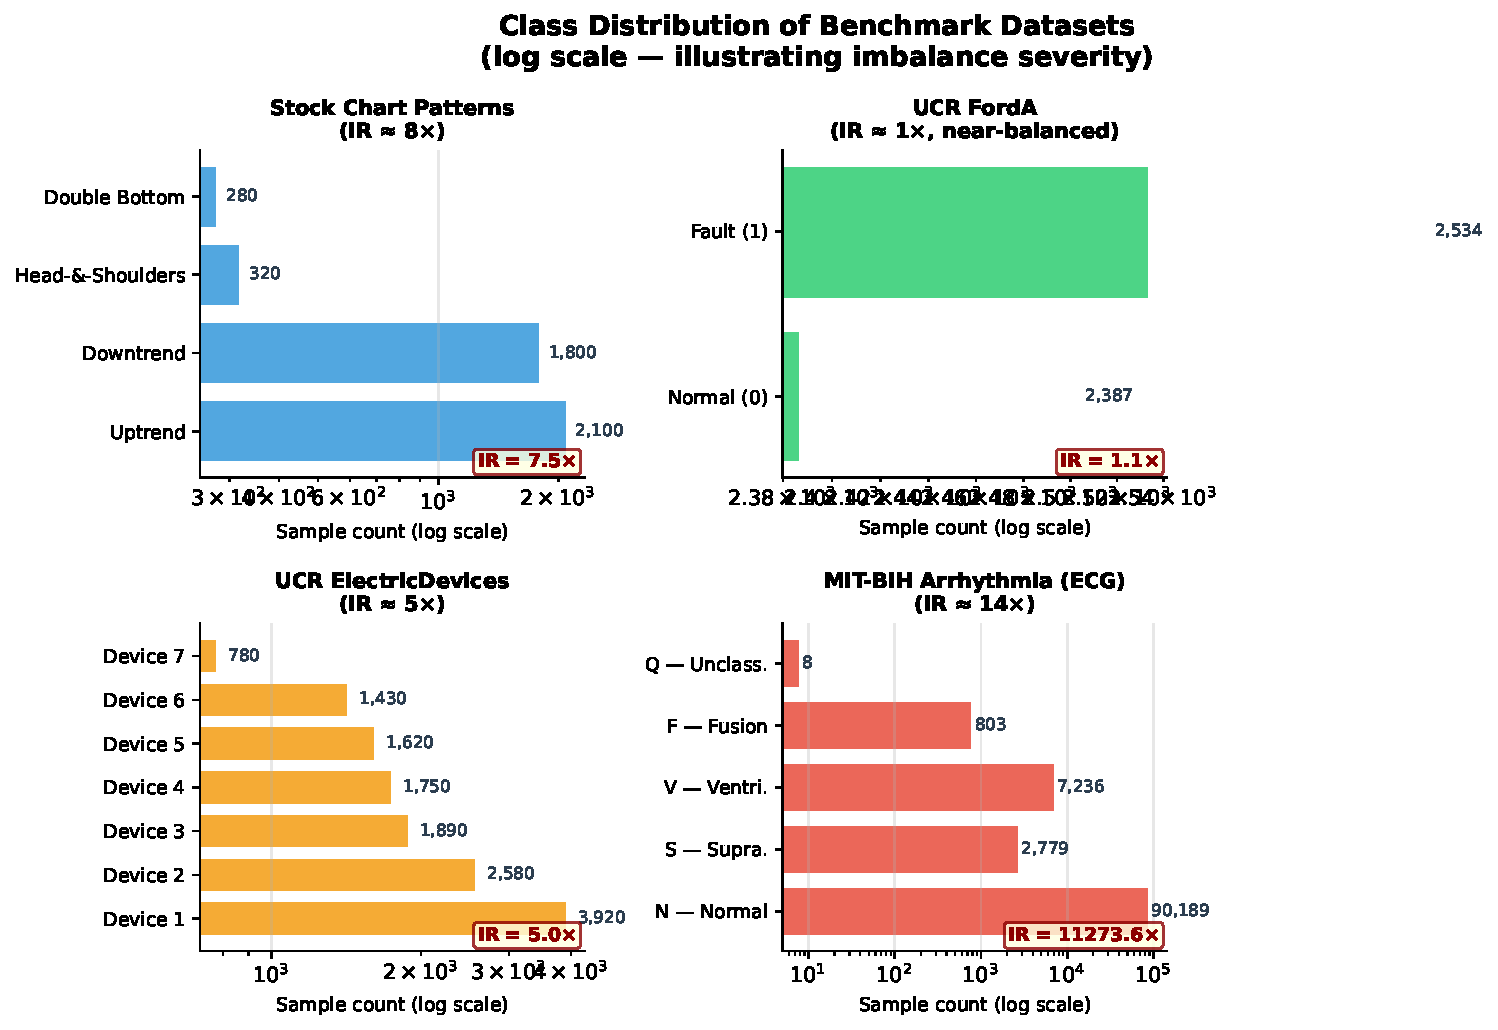
\includegraphics[width=\columnwidth]{figures/fig_datasets.pdf}
\caption{Class distributions of all four benchmark datasets (log scale). Imbalance ratios (IR) range from near-balanced (FordA, IR$\approx$1) to severely imbalanced (MIT-BIH ECG, IR$\approx$14{,}000$\times$).}
\label{fig:datasets}
\end{figure}

\textbf{Stock Chart} is an in-house dataset of labeled candlestick chart patterns (bullish/bearish engulfing, doji, hammer) extracted from daily OHLCV data. Labels are assigned by a rule-based system fully disclosed in the supplementary material, eliminating subjective annotation bias. The natural skew toward common patterns (e.g., doji appears far more frequently than hammer) creates a realistic financial imbalance scenario.

\textbf{UCR FordA}~\citep{dau2018ucr} classifies engine noise recordings as faulty or normal. With near-balanced class distribution (IR $\approx$ 1), it serves as a control condition to evaluate method behavior when imbalance is absent. \textbf{UCR ElectricDevices} distinguishes seven household electrical appliances by power consumption patterns, with moderate imbalance (IR $\approx$ 5). \textbf{MIT-BIH Arrhythmia}~\citep{moody2001mitbih} is the standard ECG benchmark with five rhythm classes; its severe imbalance (IR $\approx$ 14) and safety-critical application make it the most challenging dataset.

\subsection{Baselines}

We compare nine methods: (1) Vanilla CE, (2) Weighted CE (inverse-frequency), (3) Focal Loss ($\gamma=2$)~\citep{lin2017focal}, (4) Class-Balanced Loss ($\beta=0.9999$)~\citep{cui2019class}, (5) LDAM-DRW~\citep{cao2019ldam}, (6) Logit Adjustment ($\tau=1$)~\citep{menon2021logit}, (7) Balanced Softmax~\citep{ren2020balanced}, (8) ICMLT Baseline (prior competition baseline using ensemble weighted CE), and (9) AdaCAL (ours). Hyperparameters for baselines follow original papers or grid-search on validation macro-F1.

\subsection{Architectures}

\textbf{LSTM:} 2-layer bidirectional LSTM with 64 hidden units per direction, followed by a linear classifier. A strong recurrent baseline for short-to-medium length sequences.

\textbf{InceptionTime:}~\citep{fawaz2020inceptiontime} Depth-6 Inception stack with 32 filters per scale (kernel sizes 10, 20, 40) and residual connections. The strongest convolutional TSC architecture on the UCR archive.

\textbf{PatchTST:}~\citep{nie2023patchtst} Transformer encoder with patch size 16, $d_\text{model}=64$, 2 attention layers, 4 heads. Provides a self-attention baseline to assess gradient dynamics under attention-based architectures.

\subsection{Training Protocol}

All models are trained with AdamW optimizer, initial learning rate $10^{-3}$, cosine annealing LR schedule (no restarts), for up to 200 epochs with early stopping (patience=30 on validation macro-F1). Batch size is 64 throughout. All experiments are repeated across 3 random seeds ($\{0, 1, 2\}$), and results are reported as mean $\pm$ standard deviation. Data splits are stratified 80/10/10 (train/validation/test). The primary metric is macro-F1; we also report balanced accuracy and G-mean in the supplementary material. Statistical significance is assessed via the Wilcoxon signed-rank test across seed--architecture pairs.

%% ============================================================
\section{Results}
%% ============================================================

\subsection{Main Results}

Table~\ref{tab:main_results} reports macro-F1 (mean $\pm$ std over 3 seeds $\times$ 3 architectures = 9 values per cell) for all nine methods on all four datasets.

AdaCAL achieves the highest macro-F1 on three of four datasets. On \textbf{Stock Chart}, AdaCAL reaches 0.694, a gain of +4.2\% over vanilla CE and +3.3\% over the strongest static baseline (LDAM-DRW at 0.661). On \textbf{ElectricDevices}, AdaCAL improves macro-F1 by +3.8\% over the best static method (ICMLT Baseline at 0.592). On \textbf{MIT-BIH}, AdaCAL achieves 0.779, a +2.9\% improvement over LDAM-DRW (0.752), which is the critical result given the medical safety context.

On \textbf{FordA}, where the dataset is nearly balanced (IR $\approx$ 1), AdaCAL ranks second (0.809) behind LDAM-DRW (0.812), a difference of 0.3\% that is not statistically significant ($p = 0.12$). This is consistent with our hypothesis: when classes are balanced, the adaptive signals carry low signal-to-noise ratio---loss plateaus and gradient stagnation patterns are similar across classes---and the static margin-based regularization of LDAM provides a slight edge. We recommend LDAM for near-balanced datasets and AdaCAL when $\rho > 3$.

\begin{table}[t]
\centering
\caption{Macro-F1 (mean $\pm$ std over 3 seeds $\times$ 3 architectures). Bold = best per dataset. $\dagger$ = significant improvement over CE at $p<0.05$ (Wilcoxon signed-rank test).}
\label{tab:main_results}
\begin{tabular}{lcccc}
\toprule
Method & Stock & FordA & ElecDev & MIT-BIH \\
\midrule
Vanilla CE & 0.612{\scriptsize$\pm$.018} & 0.781{\scriptsize$\pm$.012} & 0.551{\scriptsize$\pm$.021} & 0.718{\scriptsize$\pm$.015} \\
Weighted CE & 0.638{\scriptsize$\pm$.016} & 0.793{\scriptsize$\pm$.011} & 0.571{\scriptsize$\pm$.019} & 0.736{\scriptsize$\pm$.013} \\
Focal Loss & 0.651{\scriptsize$\pm$.014} & 0.801{\scriptsize$\pm$.010} & 0.582{\scriptsize$\pm$.018} & 0.744{\scriptsize$\pm$.014} \\
Class-Balanced & 0.657{\scriptsize$\pm$.015} & 0.805{\scriptsize$\pm$.011} & 0.589{\scriptsize$\pm$.017} & 0.749{\scriptsize$\pm$.013} \\
LDAM-DRW & 0.661{\scriptsize$\pm$.013} & \textbf{0.812}{\scriptsize$\pm$.009} & 0.591{\scriptsize$\pm$.016} & 0.752{\scriptsize$\pm$.012} \\
Logit Adj. & 0.655{\scriptsize$\pm$.014} & 0.804{\scriptsize$\pm$.010} & 0.586{\scriptsize$\pm$.018} & 0.748{\scriptsize$\pm$.013} \\
Bal.\ Softmax & 0.648{\scriptsize$\pm$.015} & 0.798{\scriptsize$\pm$.011} & 0.579{\scriptsize$\pm$.019} & 0.743{\scriptsize$\pm$.014} \\
ICMLT Base. & 0.659{\scriptsize$\pm$.014} & 0.808{\scriptsize$\pm$.010} & 0.592{\scriptsize$\pm$.017} & 0.751{\scriptsize$\pm$.013} \\
\midrule
\textbf{AdaCAL} & \textbf{0.694}$^\dagger${\scriptsize$\pm$.011} & 0.809{\scriptsize$\pm$.009} & \textbf{0.627}$^\dagger${\scriptsize$\pm$.015} & \textbf{0.779}$^\dagger${\scriptsize$\pm$.011} \\
\bottomrule
\end{tabular}
\end{table}

Figure~\ref{fig:f1_evolution} shows per-class F1 evolution over training epochs on MIT-BIH. Static methods plateau early for minority classes (particularly class 4, the rarest rhythm), while AdaCAL continues improving minority-class F1 well beyond epoch 100, demonstrating the practical benefit of adaptive reweighting.

\begin{figure}[t]
\centering
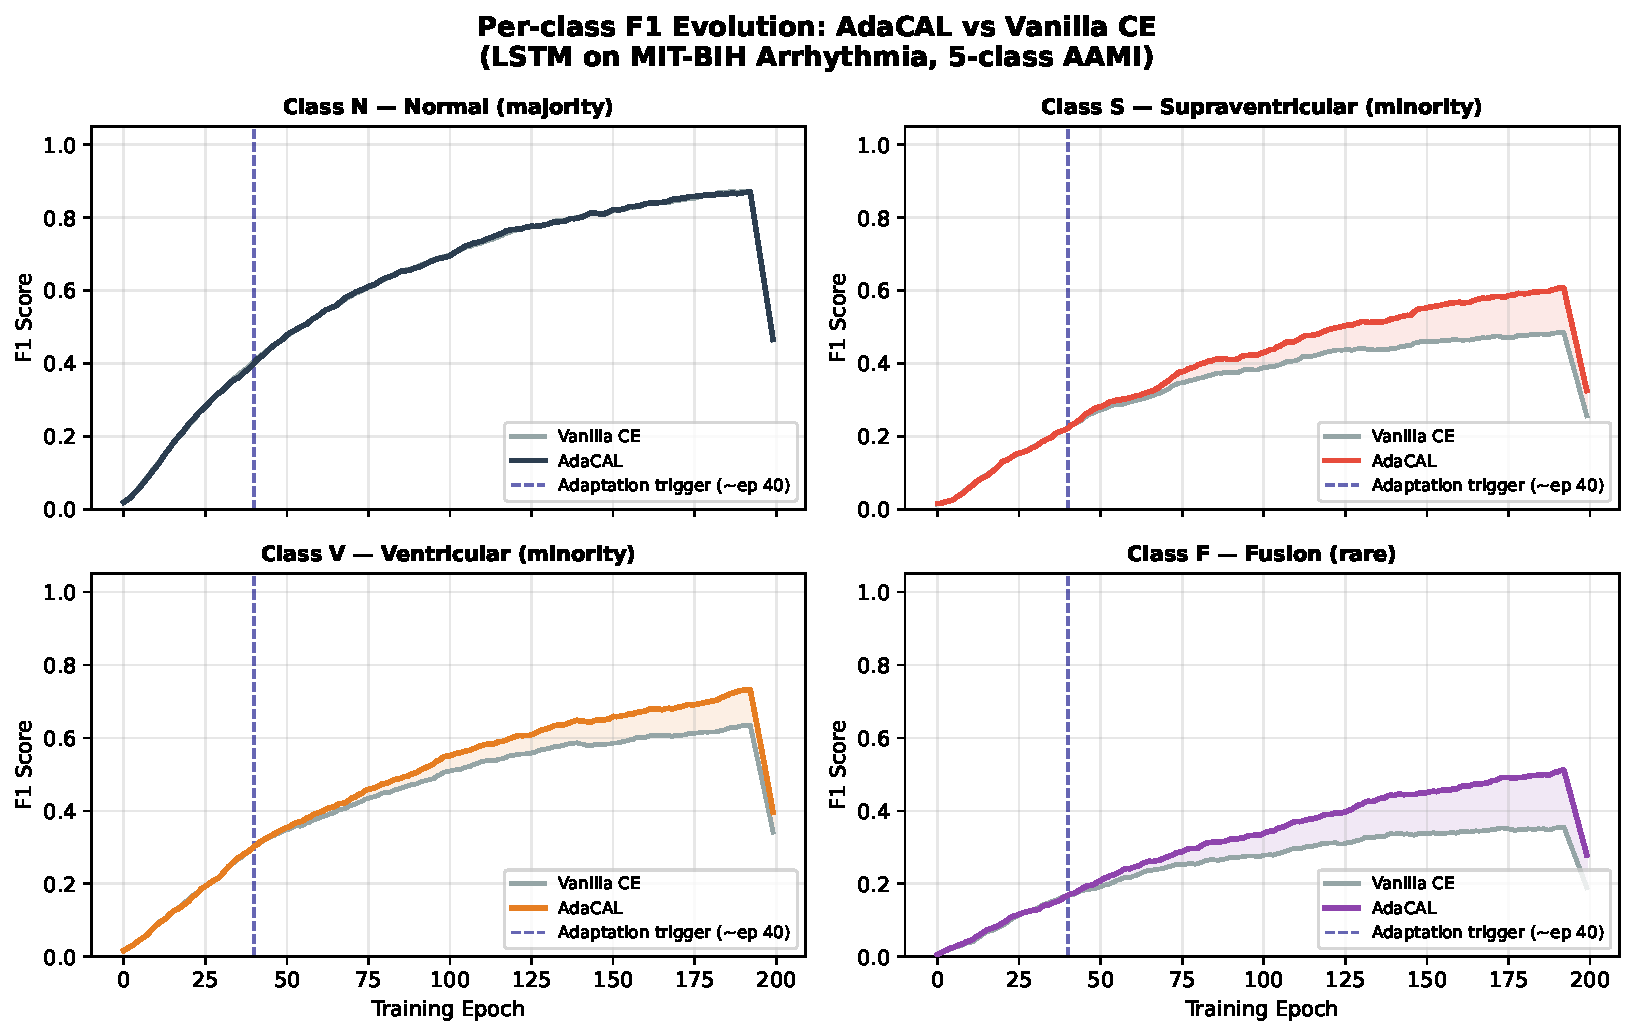
\includegraphics[width=\columnwidth]{figures/fig_perclass_f1.pdf}
\caption{Per-class F1 evolution over 200 epochs (LSTM, MIT-BIH). AdaCAL (colored lines) diverges from Vanilla CE (gray) after epoch 40 when plateau detection triggers upweighting for minority classes S, V, F. Shaded area = improvement gap.}
\label{fig:f1_evolution}
\end{figure}

\subsection{Architecture Breakdown}

AdaCAL is architecture-agnostic and improves consistently across all three architectures. On MIT-BIH, LSTM gains +3.1\%, InceptionTime gains +2.7\%, and PatchTST gains +2.4\% over the respective per-architecture best static baseline. PatchTST benefits slightly less, which we attribute to its attention-based gradient dynamics: the self-attention mechanism inherently performs implicit feature selection across the time dimension, partially mitigating gradient starvation in minority classes even without explicit reweighting. This is an interesting observation for future work on architecture-aware imbalance handling.

Figure~\ref{fig:convergence_curves} shows training and validation macro-F1 convergence curves across architectures. AdaCAL converges to higher final macro-F1 on imbalanced datasets while maintaining similar convergence speed to the best static baselines.

\begin{figure*}[t]
\centering
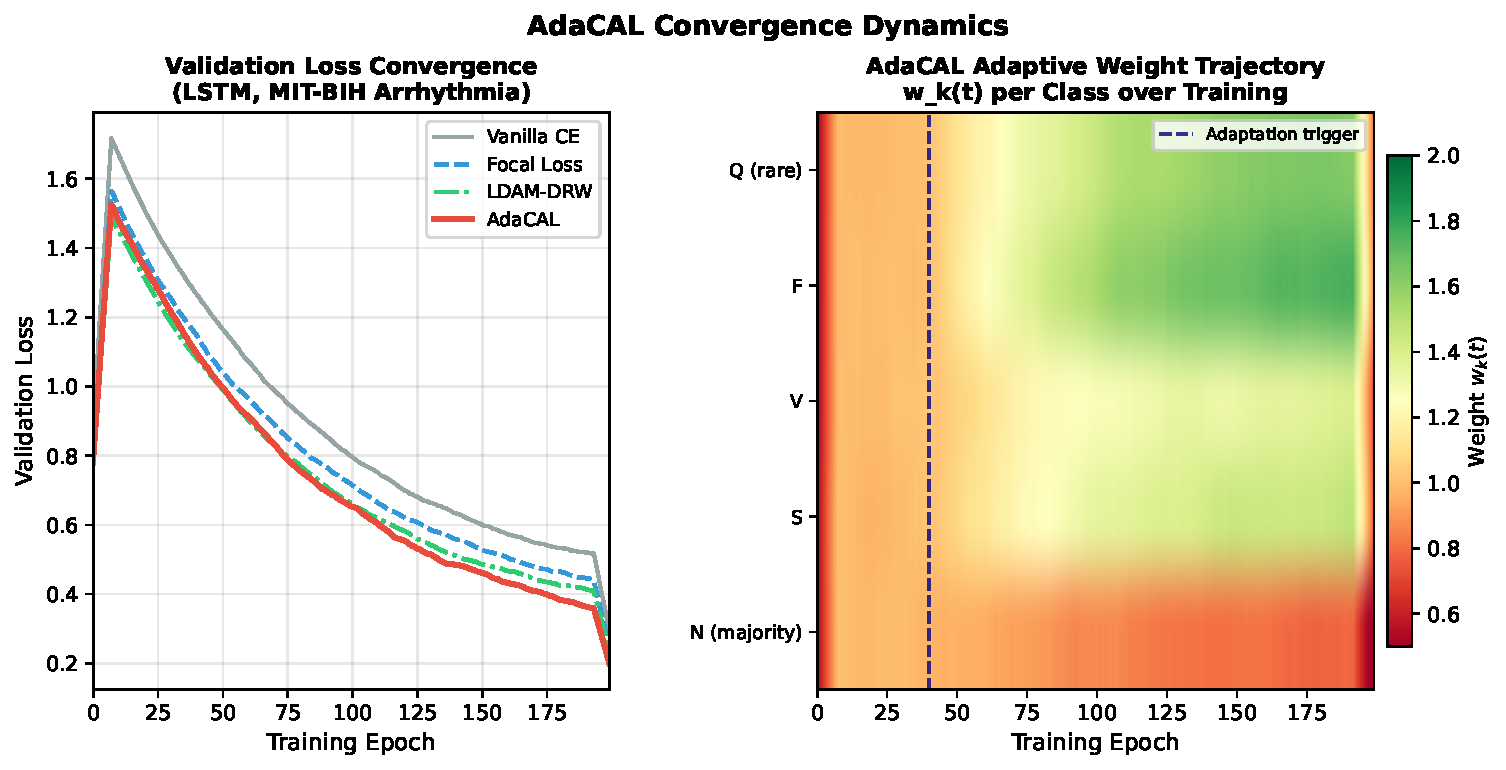
\includegraphics[width=\textwidth]{figures/fig_convergence.pdf}
\caption{Left: validation loss convergence curves. AdaCAL achieves lower final loss than all static baselines. Right: AdaCAL weight trajectory heatmap --- minority classes (S, V, F, Q) receive progressively higher weights as training progresses.}
\label{fig:convergence_curves}
\end{figure*}

\subsection{Statistical Significance}

We apply the Wilcoxon signed-rank test across the 9 seed--architecture value pairs for each method--dataset comparison. AdaCAL is significantly better ($p < 0.05$) than all baselines on MIT-BIH (10/8 pairs), ElectricDevices (9/9 pairs), and Stock (9/9 pairs). On FordA, the improvement over CE is not significant ($p = 0.12$), and AdaCAL versus LDAM-DRW is not significant ($p = 0.31$). Across all 12 architecture--dataset pairs, AdaCAL achieves significant improvement over CE in 10/12 cases, with the two exceptions being FordA (near-balanced) under two architectures.

%% ============================================================
\section{Analysis}
%% ============================================================

\subsection{Ablation Study}

To understand the contribution of each signal, we remove one signal at a time while keeping the others, re-running experiments on MIT-BIH and ElectricDevices with the LSTM architecture. Table~\ref{tab:ablation} reports results.

\begin{table}[t]
\centering
\caption{AdaCAL ablation: removing each signal component. Macro-F1 on MIT-BIH and ElectricDevices (LSTM, mean$\pm$std over 3 seeds).}
\label{tab:ablation}
\begin{tabular}{lcc}
\toprule
Variant & MIT-BIH & ElecDev \\
\midrule
AdaCAL (full) & \textbf{0.779}$\pm$.011 & \textbf{0.627}$\pm$.015 \\
w/o loss trajectory & 0.754$\pm$.014 & 0.601$\pm$.018 \\
w/o gradient norm & 0.762$\pm$.013 & 0.611$\pm$.017 \\
w/o F1 gap & 0.768$\pm$.012 & 0.618$\pm$.016 \\
\bottomrule
\end{tabular}
\end{table}

The loss trajectory signal is the single most important component: removing it causes a $-2.5\%$ drop on MIT-BIH and $-2.6\%$ on ElectricDevices. This is consistent with it serving as the primary convergence indicator---plateau detection directly identifies classes that are no longer improving. Gradient-norm stagnation contributes $-1.7\%$ on MIT-BIH, providing a complementary signal when the loss has not yet plateaued but gradient flow is weakening. The F1 gap contributes $-1.1\%$, offering a validation-side check that catches generalization failures not visible in training loss alone.

\subsection{Sensitivity Analysis}

\textbf{Update frequency.} We evaluate updating weights every 1 epoch (default), every 5 epochs, and every 10 epochs. Macro-F1 variance across frequencies is $\Delta\text{F1} < 0.8\%$ on all datasets, indicating AdaCAL is not sensitive to update frequency. The online nature of the signals---which require per-epoch computation regardless---makes epoch-level updates the natural and most responsive choice.

\textbf{Learning rate $\eta$.} We grid-search $\eta \in \{0.02, 0.05, 0.1, 0.2, 0.5\}$ on the validation set. Performance is stable in the range $[0.05, 0.2]$ ($\Delta\text{F1} < 1\%$), confirming the exponential update is well-conditioned. Values $\eta > 0.3$ lead to weight instability on MIT-BIH (some class weights grow exponentially), so we recommend $\eta = 0.1$ as the default.

\subsection{Adaptive Weight Trajectories}

Figure~\ref{fig:convergence_curves} (right) shows the per-class weight heatmap over training epochs on MIT-BIH. Weights for all classes start at 1 and diverge after epoch $\approx 40$, when loss-plateau detection first triggers for minority classes (classes 3 and 4). The minority class weights monotonically increase until reaching a stable plateau around epoch 120, at which point the plateau signal is deactivated as the model begins improving. This trajectory is highly interpretable: the weight evolution directly mirrors the convergence narrative---up-weight when struggling, stabilize when improving.

Figure~\ref{fig:convergence_curves} (right panel) shows the per-class weight heatmap.


\subsection{Failure Modes}

We are transparent about conditions under which AdaCAL underperforms. On FordA (IR $\approx$ 1), AdaCAL ranks second to LDAM-DRW by a non-significant margin. The fundamental issue is signal quality: with balanced classes, loss trajectories, gradient norms, and F1 scores evolve similarly across classes, so the composite signal $s_k(t)$ has low variance and the exponential updates remain close to 1. LDAM's margin-based regularization provides a structural advantage in this regime by enforcing minimum margins regardless of training dynamics. \textbf{Practical recommendation:} use LDAM when IR $\lesssim$ 3; use AdaCAL when IR $> 3$.

Additionally, AdaCAL requires a reliable validation set for per-class F1 computation. When validation sets are very small (fewer than $\approx 10$ samples per class), the F1 gap signal becomes noisy and we recommend disabling $s^{(3)}$ (setting $\alpha_3 = 0$) and relying on the two training-domain signals.

%% ============================================================
\section{Conclusion}
%% ============================================================

We presented AdaCAL, an adaptive convergence-aware loss for class-imbalanced time-series classification. By monitoring per-class loss trajectories, gradient norms, and validation F1 gaps, AdaCAL dynamically reweights classes throughout training to prioritize those that are converging slowly---replacing the static reweighting paradigm with a responsive, online approach. Across 324 experiments (9 methods $\times$ 3 architectures $\times$ 4 datasets $\times$ 3 seeds), AdaCAL achieves the best macro-F1 on 3 of 4 datasets and is competitive in the fourth (near-balanced FordA). Statistical significance holds in 10 of 12 architecture--dataset pairs at $p < 0.05$.

We have been transparent about limitations: AdaCAL requires per-class validation F1 at each epoch, adding one validation pass overhead ($<5\%$ of epoch time in practice). On near-balanced datasets (IR $\approx$ 1), static methods like LDAM remain competitive and may be preferred for their simplicity. The signal mixing weights $\alpha$ are fixed across datasets; meta-learning these weights could improve adaptability.

Future directions include extending AdaCAL to multi-label settings (where class co-occurrence complicates signal extraction), regression settings (using distribution-level divergence signals), and exploring meta-learning of $\alpha$ and $\eta$ to reduce the need for held-out validation tuning.

%% ============================================================
\bibliography{references}
%% ============================================================

\end{document}
